\subsection{Differential analysis on QR function}
\begin{frame}
\frametitle{Differential analysis on QR function}
As $QR(X)\rightarrow y$ and we get $X^\prime$ by flipping some random bits of $X$. \\
As $n$ increases, $m$ tend towards the expected equilibrium of half the length of $Y$. Analysis based on measuring $HD ( QR (x^\prime), \ y)$ : 


\setlength{\columnsep}{10pt}
\begin{multicols}{2}
\setlength{\leftmargin}{1pt}

{\begin{itemize}
    \item \small{The bit flipping is given by $x$-axis. i.e. $n$ times.}
    \item \small{The $HD$ between $2$ values are given by $y$-axis.}
    \item \small{Legend of the Plot : }
    \begin{enumerate}
    \setcounter{enumi}{-1} % Set the counter to start from 0
        \item  \scriptsize{$HD(X,Y)$}
        \item  \scriptsize{Convergence point of the Hamming distance between two random values}
        \item \scriptsize{$HD(Y,Y^\prime)$}
        \item \scriptsize{$HD(X,X')$}
        \item[] \scriptsize{Assuming $HD(X,X^\prime) < \ \frac{key \ size}{8}$, $HD(X,\ X^\prime)$ should be easily distinguishable.}
    \end{enumerate}
\end{itemize}}

\columnbreak
\setlength{\rightmargin}{0pt}
\begin{figure}
    \centering
    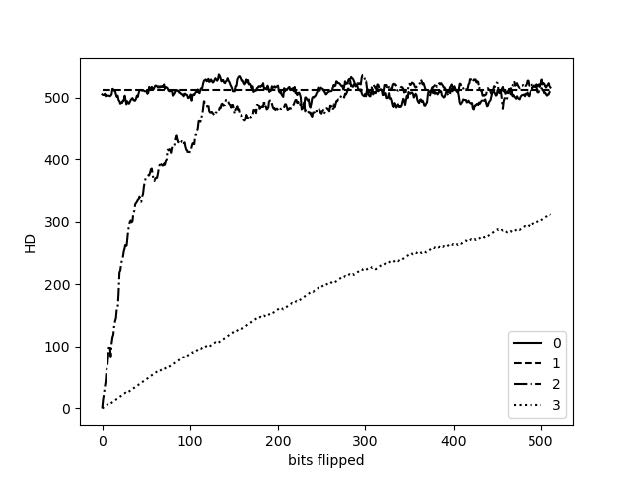
\includegraphics[scale=0.52]{fig1.jpg}
    \caption{Flipping of random bits in $X$}
\end{figure}

\end{multicols}

\end{frame}